\documentclass[a4paper,10pt]{article}

\usepackage[brazilian]{babel}
\usepackage[left=2.5cm,right=2.5cm,top=3cm,bottom=2.5cm]{geometry}
\usepackage{mathtools}
\usepackage{amsthm}
\usepackage{amsmath}
%\usepackage{nccmath}
\usepackage{amssymb}
\usepackage{amsfonts}
\usepackage{physics}
%\usepackage{dsfont}
%\usepackage{mathrsfs}

\usepackage{titling}
\usepackage{indentfirst}

\usepackage{bm}
\usepackage[dvipsnames]{xcolor}
\usepackage{cancel}

\usepackage{xurl}
\usepackage[colorlinks=true]{hyperref}

\usepackage{float}
\usepackage{graphicx}
%\usepackage{tikz}
\usepackage{caption}
\usepackage{subcaption}

%%%%%%%%%%%%%%%%%%%%%%%%%%%%%%%%%%%%%%%%%%%%%%%%%%%

\newcommand{\eps}{\epsilon}
\newcommand{\vphi}{\varphi}
\newcommand{\cte}{\text{cte}}

\newcommand{\N}{\mathbb{N}}
\newcommand{\Z}{\mathbb{Z}}
\newcommand{\Q}{\mathbb{Q}}
\newcommand{\R}{\vb{R}}
\newcommand{\C}{\mathbb{C}}
\renewcommand{\S}{\hat{S}}
%\renewcommand{\H}{\s{H}}

\renewcommand{\a}{\vb{a}}
\newcommand{\nn}{\hat{n}}
\renewcommand{\d}{\dagger}
\newcommand{\up}{\uparrow}
\newcommand{\down}{\downarrow}

\newcommand{\0}{\vb{0}}
%\newcommand{\1}{\mathds{1}}
\newcommand{\E}{\vb{E}}
\newcommand{\B}{\vb{B}}
\renewcommand{\v}{\vb{v}}
\renewcommand{\r}{\vb{r}}
\renewcommand{\k}{\vb{k}}
\newcommand{\p}{\vb{p}}
\newcommand{\q}{\vb{q}}
\newcommand{\F}{\vb{F}}

\newcommand{\s}{\sigma}
%\newcommand{\prodint}[2]{\left\langle #1 , #2 \right\rangle}
\newcommand{\cc}[1]{\overline{#1}}
\newcommand{\Eval}[3]{\eval{\left( #1 \right)}_{#2}^{#3}}

\newcommand{\unit}[1]{\; \mathrm{#1}}

\newcommand{\n}{\medskip}
\newcommand{\e}{\quad \mathrm{e} \quad}
\newcommand{\ou}{\quad \mathrm{ou} \quad}
\newcommand{\virg}{\, , \;}
\newcommand{\ptodo}{\forall \,}
\renewcommand{\implies}{\; \Rightarrow \;}
%\newcommand{\eqname}[1]{\tag*{#1}} % Tag equation with name

\setlength{\droptitle}{-7em}

\theoremstyle{plain}
\newtheorem{theorem}{Teorema}[section]
%\newtheorem{defi}[theorem]{Definição}
\newtheorem{lemma}[theorem]{Lema}
%\newtheorem{corol}[theorem]{Corolário}
%\newtheorem{prop}[theorem]{Proposição}
%\newtheorem{example}{Exemplo}
%
%\newtheorem{inneraxiom}{Axioma}
%\newenvironment{axioma}[1]
%  {\renewcommand\theinneraxiom{#1}\inneraxiom}
%  {\endinneraxiom}
%
%\newtheorem{innerpostulado}{Postulado}
%\newenvironment{postulado}[1]
%  {\renewcommand\theinnerpostulado{#1}\innerpostulado}
%  {\endinnerpostulado}
%
%\newtheorem{innerexercise}{Exercício}
%\newenvironment{exercise}[1]
%  {\renewcommand\theinnerexercise{#1}\innerexercise}
%  {\endinnerexercise}
%
%\newtheorem{innerthm}{Teorema}
%\newenvironment{teorema}[1]
%  {\renewcommand\theinnerthm{#1}\innerthm}
%  {\endinnerthm}
%
\newtheorem{innerlema}{Lema}
\newenvironment{lema}[1]
  {\renewcommand\theinnerlema{#1}\innerlema}
  {\endinnerlema}
%
%\theoremstyle{remark}
%\newtheorem*{hint}{Dica}
%\newtheorem*{notation}{Notação}
%\newtheorem*{obs}{Observação}


\newcommand{\vac}{\ket{vac}}
\newcommand{\hh}{\tilde{h}}
\newcommand{\hhh}{\bm{\tilde{h}}}
\newcommand{\vecs}{(\s^x, \s^y, \s^z)}
\renewcommand{\ss}{\bm{\sigma}}


\title{\Huge{\textbf{Lista 5 - Mecânica Estatística}}}
\author{Mateus Marques}

\begin{document}

\maketitle

\section*{1) Paredes de domínio}

(a) Na teoria de Ginzburg-Landau para Ising, a energia livre é escrita (em dimensão $d=1$) como
$$
F = \int \dd[d]{\vb{x}} \qty{-\frac{c}{2} \phi(\vb{x}) \nabla^2 \phi(\vb{x}) + f[\phi(\vb{x})] - h \phi(\vb{x})} = \int \dd{x} \qty{-\frac{c}{2} \phi(x) \dv[2]{x} \phi(x) + f[\phi(x)] - h \phi(x)},
$$
onde $\phi$ faz o papel da magnetização e $f(\phi) = \frac{1}{2} r \phi^2 + u \phi^4$.

\n

Extremizando a energia livre, temos que
$$
0 = \fdv{F}{\phi} = -c \, \dv[2]{\phi}{x} + \dv{f[\phi(x)]}{\phi} - h.
$$

No limite de campo infinitesimal $h \to 0$ obtemos
$$
\boxed{ c \, \dv[2]{\phi}{x} = \dv{f[\phi(x)]}{\phi} = r \phi + 4u \phi^3. }
$$

Essa equação é análoga à segunda lei de Newton
$$
m \dv[2]{x}{t} = - \dv{V}{x},
$$
com as identificações $t \leftrightarrow x$, $x \leftrightarrow \phi$, $m \leftrightarrow c$ e $V(x) \leftrightarrow -f(\phi)$. A Figura \ref{fig:hill} mostra a colina de potencial nesta analogia.
\begin{figure}[H]
\centering
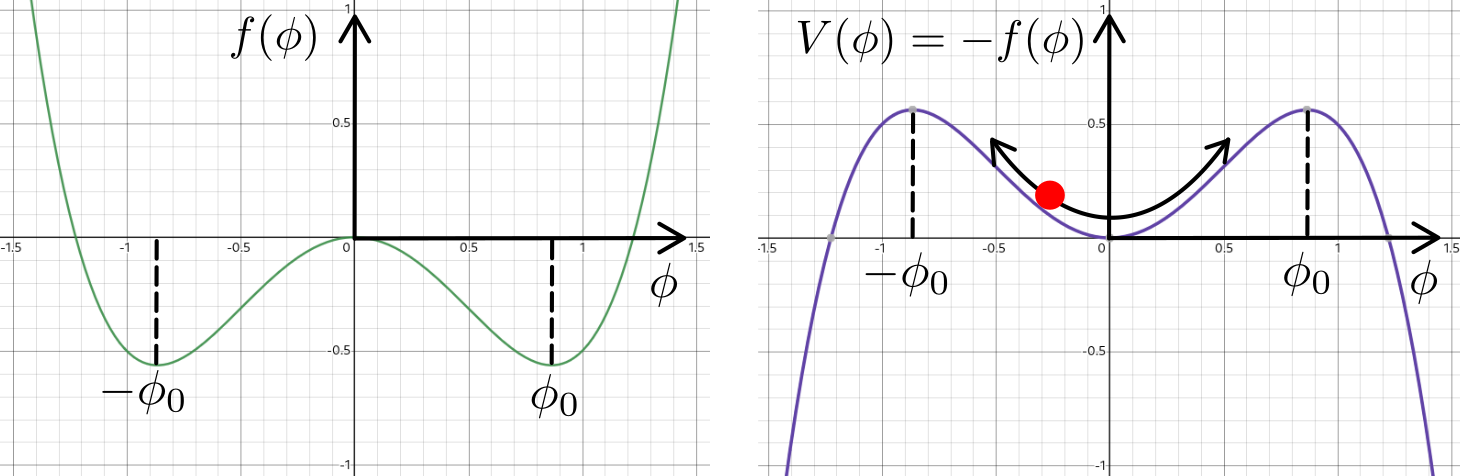
\includegraphics[width=0.9\linewidth]{fig/hill.png}
\caption{Colina de potencial $V(\phi) = -f(\phi)$.}
\label{fig:hill}
\end{figure}

\n\n

(b) Multiplicando a equação obtida por $\dd{\phi}/\dd{x}$, reconhecendo a regra da cadeia e assumindo que a energia do sistema (newtoniano) seja $E = V(\phi_0) = -f(\phi_0)$, temos
$$
\dv{x}\qty{\frac{c}{2} \qty(\dv{\phi}{x})^2 - f[\phi(x)]} = 0 \implies
\qty(\dv{\phi}{x})^2 = \frac{2}{c} \, [f(\phi) - f(\phi_0)].
$$

Lembre que $\phi_0$ é um mínimo da função $f(\phi) =  \frac{1}{2} r \phi^2 + u \phi^4$, de maneira que $\phi_0^2 = -r/4u$ e
$$
\qty(\dv{\phi}{x})^2 = \frac{2}{c} \, [f(\phi) - f(\phi_0)] = \frac{2}{c} \frac{(r + 4 u \phi^2)^2}{16 u}
= \frac{r^2}{8 \, cu} \qty(1 - \frac{\phi^2}{\phi_0^2} )^2 \implies
\boxed{ \dv{\phi}{x} = \sqrt{\frac{r^2}{8 \, cu}} \qty( 1 - \frac{\phi^2}{\phi_0^2} ). }
$$

Assumindo que $\phi(0) = 0$ (a parede de domínio está localizada em $x = 0$), temos
$$
\int_0^{\phi} \frac{\dd{\phi}}{1 - \qty(\frac{\phi^2}{\phi_0^2}) } = \sqrt{\frac{r^2}{8 \, cu}} \, \int_0^x \dd{x} \implies
\phi_0 \, \tanh[-1](\frac{\phi}{\phi_0}) = \sqrt{\frac{r^2}{8 \, cu}} \, x = \phi_0 \sqrt{\frac{-r}{2c}} \, x \implies
$$
$$
\frac{\phi}{\phi_0} = \tanh(\sqrt{\frac{-r}{2c}} \, x) \implies
\boxed{ \phi(x) = \phi_0 \tanh(\frac{x}{\sqrt{2} \, \xi}), }
$$
onde $\xi = \sqrt{-c/r}$ é o comprimento de correlação. O esboço (Figura \ref{fig:soliton}) dessa solução já foi feita na própria lista de exercícios.
\begin{figure}[H]
\centering
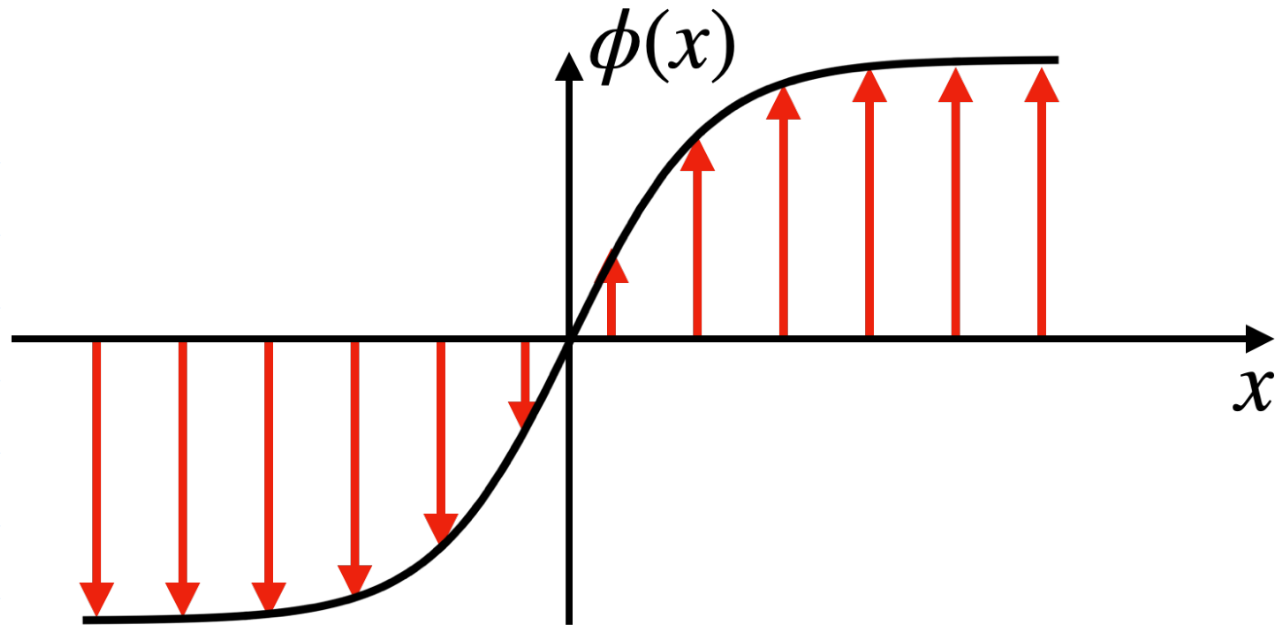
\includegraphics[width=0.6\linewidth]{fig/soliton.png}
\caption{Esboço da solução sóliton para a parede de domínio.}
\label{fig:soliton}
\end{figure}

A solução do sóliton descreve bem uma parede de domínio que leva uma distância infinita para ter os spins alinhados. Note que na localização $x = 0$ os spins mudam de direção, e eles somente se alinham totalmente em $x \to \pm \infty$, em que $\displaystyle{\lim_{x\to\pm\infty} \abs{\phi(x)} = 1}$.

\n

(c) A energia livre da solução sóliton é (lembrando que $A = \int \dd[d-1]{\vb{x}}$ é a área)
$$
F = \int \dd[d]{\vb{x}} \qty{-\frac{c}{2} \phi(\vb{x}) \nabla^2 \phi(\vb{x}) + f[\phi(\vb{x})]} =
A \int \dd{x} \qty[-\frac{c}{2} \phi \, \dv[2]{\phi}{x} + f(\phi)] =
$$
$$
= A \int \dd{x} \qty[-\frac{1}{2} \phi \, \qty(r\phi + 4u \phi^3) + \frac{r}{2} \phi^2 + u \phi^4]
= -Au \int \dd{x} \phi^4(x).
$$

A energia livre da fase ordenada $\phi(x) = \phi_0 = \sqrt{-r/4u}$, $f(\phi_0) = -\frac{r^2}{16u} = -u \phi_0^4$, é
$$
F_0 = A \int \dd{x} \qty[-\cancelto{0}{\frac{c}{2} \phi \, \dv[2]{\phi}{x}} + f(\phi)] = A \int \dd{x} f(\phi_0) =
-A u \int \dd{x} \phi_0^4.
$$

Portanto a contribuição da parede de domínio é
$$
\boxed{\Delta F = F - F_0 = Au \int \dd{x} \Big[\phi_0^4 - \phi^4(x)\Big].}
$$

\n

A tensão superficial é dada por (substituindo $y = x/\sqrt{2} \xi$)
$$
\s = \frac{\Delta F}{A} = u \phi_0^4 \int_{-\infty}^{\infty} \dd{x} \qty[1 - \tanh(\frac{x}{\sqrt{2} \xi})^4] =
\sqrt{2} u \xi \phi_0^4 \int_{-\infty}^{\infty} \dd{y} \qty[1 - \tanh(y)^4].
$$

O Mathematica resolveu a integral $\int_{-\infty}^{\infty} \dd{y} \qty[1 - \tanh(y)^4] = 8/3$. Finalmente, obtemos que
$$
\boxed{\s = \frac{8\sqrt{2}}{3} \xi u \phi_0^4 = \frac{\sqrt{8}}{3} \xi u' \phi_0^4.}
$$

A tensão superficial está diferente da lista $\s' = \frac{\sqrt{8}}{3} \xi u \phi_0^4$ por um fator de $4$. Acredito que o resultado da lista dependa da definição $f'(\phi) = \frac{1}{2} r\phi^2 + \frac{u'}{4} \phi^4$, onde $\boxed{u = u'/4}$ e eu defini $f(\phi) = \frac{1}{2} r\phi^2 + u \phi^4$.


\pagebreak


\section*{4) Grupo de renomalização em uma dimensão}

(a) Considerando o sítio $S_1$, que é conectado aos sítios 0 e 2, temos para os parâmetros renormalizados $K$ e $F$
$$
e^{K'S_0 S_2 + F} = \sum_{S_1 = \pm 1} e^{K S_1(S_0 + S_2)} = e^{K(S_0+S_2)} + e^{-K(S_0+S_2)}.
$$

Como a igualdade acima deve valer para quaisquer spins $S_0 = \pm 1$ e $S_2 = \pm 1$, temos para $S_0 = S_1 = 1$ que
$$
e^{K'} e^{F} = e^{2K} + e^{-2K} = 2 \cosh(2K),
$$
e para $S_0 = 1$ e $S_2 = -1$
$$
e^{-K'} e^{F} = e^0 + e^0 = 2.
$$

Portanto:
$$
\boxed{ e^{2K'} = (e^{K'}e^{F}) (e^{K'}e^{-F}) = 2 \cosh(2K) \cdot \frac{1}{2} = \cosh(2K), }
$$
$$
e^{2F} =  (e^{K'}e^{F}) (e^{-K'}e^{F}) = 2 \cosh(2K) \cdot 2 = 4 \cosh(2K).
$$

Esse argumento não vale apenas para o sítio $S_1$, ele é geral. Podemos ver isso removendo os sítios ímpares e estudando a função de partição:
$$
Z(K) =
$$
$$
= \sum_{S_j = \pm 1} e^{K \sum_{j=-\infty}^{\infty} S_j S_{j+1}}
= \sum_{S_{2j} = \pm 1} \sum_{S_{2j + 1} = \pm 1}
\Big[
\cdots
\Big( e^{K S_{2j-2} S_{2j-1} + S_{2j-1} S_{2j}} \Big)
\Big( e^{K S_{2j} S_{2j+1} + S_{2j+1} S_{2j+2}} \Big)
\cdots
\Big]
$$
$$
= \sum_{S_{2j} = \pm 1}
\qty{
\cdots
\qty[ \sum_{S_{2j-1} = \pm 1} e^{K S_{2j-2} S_{2j-1} + S_{2j-1} S_{2j}} ]
\qty[ \sum_{S_{2j+1} = \pm 1} e^{K S_{2j} S_{2j+1} + S_{2j+1} S_{2j+2}} ]
\cdots
}
$$
$$
= \sum_{S_{2j} = \pm 1}
\qty{
\cdots
\qty[ \sum_{S_{2j-1} = \pm 1} e^{K S_{2j-1} (S_{2j-2} + S_{2j})} ]
\qty[ \sum_{S_{2j+1} = \pm 1} e^{K S_{2j+1} (S_{2j} + S_{2j+2})} ]
\cdots
}
$$
$$
= \sum_{S_{2j} = \pm 1}
\qty{
\cdots
\Big[e^{K'S_{2j-2} S_{2j} + F}\Big]
\Big[e^{K'S_{2j} S_{2j+2} + F}\Big]
\cdots
}
$$
$$
= \sum_{S_{2j} = \pm 1} \exp\qty{ \sum_{j=-\infty}^{j=\infty} \Big[K' S_{2(j-1)}S_{2j} + F\Big] }.
$$

Isso mostra que a renormalização dos parâmetros $K'$ e $F$ não depende do sítio.

\n\n

Usando a equação $2 e^{2K'} = e^{2K} + e^{-2K}$, temos
$$
\tanh^2 K = \frac{(e^K - e^{-K})^2}{(e^K + e^{-K})^2} = \frac{e^{2K} + e^{-2K} - 2}{e^{2K} + e^{-2K} + 2} =
\frac{2e^{2K'} - 2}{2e^{2K'} + 2} = \frac{e^{K'} - e^{-K'}}{e^{K'} + e^{-K'}} = \tanh(K'),
$$
o que mostra que a equação para $K'$ pode ser escrita como
$$
\boxed{ \tanh(K') = \tanh^2 K. }
$$

\n

Nas notas de aula vimos que o comprimento de correlação $\xi(K)$ é definido
$$
\xi(K) = \frac{-1}{\log(\tanh K)}.
$$

\n

Quando retiramos metade dos sítios, temos que
$$
\xi(K') = \frac{-1}{\log(\tanh K')} = \frac{-1}{\log(\tanh^2 K)} = \frac{-1}{2 \log(\tanh K)} = \frac{1}{2} \, \xi(K).
$$

\n\n

(b) Os pontos fixos $K^*$ são determinados por
$$
\tanh^2 K^* = \tanh K^* \implies \tanh K^* (\tanh K^* - 1) = 0 \implies \boxed{ K^* = 0 \ou K^* = +\infty.}
$$

\n

Lembrando que $K = \beta J$, o ponto $K^* = 0$ corresponde a $T \to +\infty$ e $K^* = +\infty$ corresponde a $T = 0$.

\n

Analisaremos a estabilidade dos dois pontos $K = 0$ e $K = +\infty$:

\n

Note que, para $K$ finito, $\tanh(K)$ tem módulo menor que 1. Assim, pela equação $\tanh(K') = \tanh^2 K$, a cada etapa de renormalização $\tanh(K)$ vai diminuindo seu módulo. No limite do infinito, teremos que $\tanh(K) \to 0 \implies K \to 0$. Isso mostra que o ponto $K = 0$ é estável, pois a renormalização iterativa faz $K \to 0$. Isso também mostra que o ponto $K = +\infty$ é instável, pois para qualquer $K$ finito a renormalização fará $K$ tender a zero, se afastando sempre do ponto $K = +\infty$.

\n

Fisicamente, a renormalização fazer $K \to 0$ nos mostra que, para qualquer $T > 0$, para flutuações de longa distância o sistema se comporta como $K$ fosse igual a zero, ou seja, como se a temperatura fosse infinita e que o sistema está na fase paramagnética (como sabemos pela solução exata em uma dimensão). Agora, para $K = +\infty$ isso mostra que a fase ferromagnética trivial em $T = 0$ (que é a temperatura crítica do modelo de Ising em 1D) é destruída para qualquer $T > 0$, ou seja, é instável.




\pagebreak

\section*{6) Modelo de Ising em um campo transverso}

(a) Este modelo é verdadeiramente quântico pois ele trata os spins como operadores quânticos (representados pelas matrizes de Pauli), diferentemente do modelo de Ising usual que os trata como variáveis binárias $\pm 1$.

\n

Considerando $T = 0$ e olhando a hamiltoniana em 1D
$$
H = -J \sum_{j} \s_j^x \s_{j+1}^x - h \sum_{j} \s_j^z,
$$
podemos imaginar o que acontece nos limites $h/J \gg 1$ e $h/J \ll 1$:
\begin{itemize}
\item $h / J \gg 1$: Neste limite só a direção $z$ importa e temos um ground-state ferromagnético $\ket{\up\up\up\cdots}$.

\item $h / J \ll 1$: Neste limite só a direção $x$ importa. O ground-state é degenerado, podendo ser combinações lineares de $\ket{\rightarrow\rightarrow\rightarrow\cdots}$ e $\ket{\leftarrow\leftarrow\leftarrow\cdots}$. Porém note que não há nenhuma preferência quanto ao eixo $z$. Isso define uma fase paramagnética.
\end{itemize}

As duas fases ferromagnética ($h/J \gg 1$) e paramagnética ($h/J \ll 1$) devem ser separadas por uma transição que depende do parâmetro de ordem $h/J$, o que configura uma transição de fase em $T = 0$, ou seja, implica na existência de um ponto crítico quântico.

\n

O diagrama de fase em $T = 0$ é esquematizado na Figura \ref{fig:qcp} abaixo.
\begin{figure}[H]
\centering
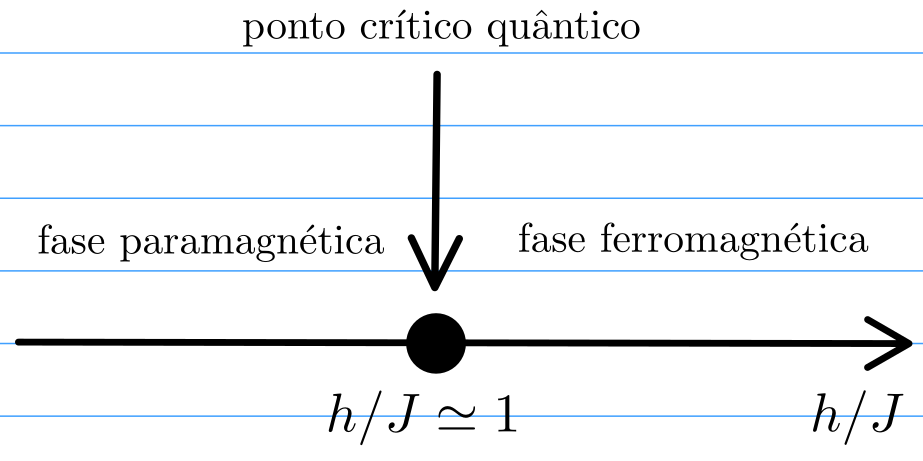
\includegraphics[width=0.8\linewidth]{fig/qcp.png}
\caption{Diagrama de fase com transição de fase quântica em $T=0$.}
\label{fig:qcp}
\end{figure}

\n\n

(b) Utilizaremos teoria de perturbação para $J \to 0$. Primeiramente, quando $J$ é exatamente zero, o estado fundamental é $\vac = \ket{\cdots\up\up\up\up\cdots}$, onde todos os $N$ spins apontam para cima. Nesse caso $J = 0$, a energia dele é $E_0 = -h N$. Agora, considerando uma aproximação apenas de primeira ordem em $J$, as excitações de partícula única são quando apenas um spin no sítio $i$ aponta para baixo, enquanto todos os outros continuam apontando para cima. Chamaremos o estado dessa excitação de $\ket{i}$. Note que se um spin no sítio $j$ está virado para cima, aplicar o operador $\s_j^x$ faz com que ele vire para baixo. Por isso, temos que $\ket{i} = \s_i^x \vac$.

\n

Agora nós consideraremos o subespaço desses estados de excitação de partícula única, em que seu projetor ortogonal ($P^2 = P$, $P^\d = P$) é dado por
$$
P = \sum_{i} \dyad{i} = \sum_{i} \s_i^x \dyad{vac} \s_i^x.
$$

\n

No formalismo de perturbação de primeira ordem, consideraremos a hamiltoniana restrita a este subespaço e a diagonalizaremos. Substraindo a energia do estado fundamental, temos então que a hamiltoniana das excitações de partícula única é
$$
H' = P(H - E_0) P = P H_0 P + P V P - E_0 P,
$$
onde $H = H_0 + V$, $H_0 = -h \sum_{j} \s_j^z$ e $V = -J \sum_{j} \s_j^x \s_{j+1}^x$.

\n\n

É fácil ver que os estados $\ket{i}$ são autoestados de $H_0$, com energia $E_0 + 2 h = -h (N-2)$ (virar um spin para baixo custa $2h$ de energia). Temos então
$$
P H_0 P = (E_0 + 2h) P = (E_0 + 2h) \sum_{j} \dyad{j}.
$$

\n

Para a perturbação $V$, temos que
$$
PVP =
\qty(
\sum_{i} \dyad{i}
)
\qty(
-J \sum_{j} \s_j^x \s_{j+1}^x
)
\qty(
\sum_{k} \dyad{k}
)
$$
$$
PVP =
-J \sum_{ijk} \ket{i}
\Big(
\mel{i}{\s_j^x \s_{j+1}^x}{k}
\Big)
\bra{k}.
$$

\n

O elemento de matriz de interesse é $\mel{i}{\s_j^x \s_{j+1}^x}{k}$. Analisaremos ele caso a caso:
\begin{itemize}
\item $i = j$. Nesse caso, o operador $\s_j^x$ vira o spin $\down$ no sítio $i$ de volta para cima. Isso nos dá que $\s_j^x \ket{i} = \s_j^x \ket{j} = \vac$. Assim, temos que
$$
\mel{i}{\s_j^x \s_{j+1}^x}{k} = \mel{vac}{\s_{j+1}^x}{k} = \braket{j+1}{k} = \delta_{j+1,k}.
$$
\item $i = j+1$. Esse caso é parecido com anterior. Lembre-se que matrizes de Pauli de sítios diferentes comutam. Portanto
$$
\mel{i}{\s_j^x \s_{j+1}^x}{k} = \mel{i}{\s_{j+1}^x \s_j^x}{k} = \mel{j+1}{\s_{j+1}^x \s_j^x}{k}
= \mel{vac}{\s_{j}^x}{k} = \braket{j}{k} = \delta_{j,k}.
$$
\item $i \neq j$ e $i \neq j+1$. Como o sítio em $i$ é diferente dos sítios $j$ e $j+1$, temos $\s_{j+1}^x \s_j^x \ket{i} = \ket{i, j, j+1}$, que denota o estado de muitos corpos onde há 3 sítios diferentes ($i$, $j$ e $j+1$) com spins $\down$ e todos os outros sítios possuem spins $\up$. Portanto, nesse caso temos
$$
\mel{i}{\s_j^x \s_{j+1}^x}{k} = \braket{i,j,j+1}{k} = 0,
$$
pois o estado $\ket{k}$ só possui um spin $\down$, que é ortogonal a $\ket{i,j,j+1}$, que possui três spins $\down$.
\end{itemize}

Interpolando os três casos analisados, concluimos que
$$
\mel{i}{\s_j^x \s_{j+1}^x}{k} = \delta_{ij} \delta_{j+1, k} + \delta_{i,j+1} \delta_{jk}.
$$

Assim, temos
$$
PVP =
-J \sum_{ijk} \ket{i}
\Big(
\delta_{ij} \delta_{j+1, k} + \delta_{i,j+1} \delta_{jk}
\Big)
\bra{k} =
$$
$$
=
-J \sum_{ijk} \ket{i} \delta_{ij} \delta_{j+1, k} \bra{k}
-J \sum_{ijk} \ket{i} \delta_{i,j+1} \delta_{jk} \bra{k}
\implies
$$
$$
PVP =
-J \sum_{j} \Big(
\dyad{j}{j+1} + \dyad{j+1}{j}
\Big).
$$

\n

Portanto, a hamiltoniana das excitações de partícula única (em primeira ordem em $J$) é
$$
\boxed{
H' = P(H_0 + V - E_0)P =
2h \sum_{j} \dyad{j}
-J \sum_{j} \Big(
\dyad{j}{j+1} + \dyad{j+1}{j}
\Big).
}
$$

\n

Perceba que $H'$ é um hamiltoniano de \textit{tight-binding} em 1D no subespaço dos estados $\ket{i}$. É um hamiltoniano muito comum na \textbf{Física do Estado Sólido}, que pode ser diagonalizado no espaço de momentos da Primeira Zona de Brillouin (BZ), que no caso 1D com parâmetro de rede $a$ é o intervalo de momentos $-\pi/a \leq k < \pi/a$.
$$
\ket{k}_{\text{BZ}} =
\frac{1}{\sqrt{N}} \sum_{j} e^{-ika j} \ket{j} \implies
\ket{j} =
\frac{1}{\sqrt{N}} \sum_{k \in \text{BZ}} e^{ika j} \ket{k} .
$$

\n

Reescrevendo a hamiltoniana $H$ em termos dos estados de momento, é fácil diagonalizá-la (esse é um cálculo direto e muito frequentemente feito em Estado Sólido):
$$
H' =
\sum_{k \in \text{BZ}}
\Big(2h - 2J \cos ka\Big) \dyad{k} =
\sum_{k \in \text{BZ}}
\eps(k) \dyad{k}.
$$

\n

A perturbação de primeira ordem nos mostra então que as excitações de partícula única são
$$
\eps(k) = 2h - 2J \cos ka + O(J^2).
$$

\n

Graficando essa relação de dispersão para diferentes valores de $h/J$, obtemos a Figura \ref{fig:transv_ising} abaixo.
\begin{figure}[H]
\centering
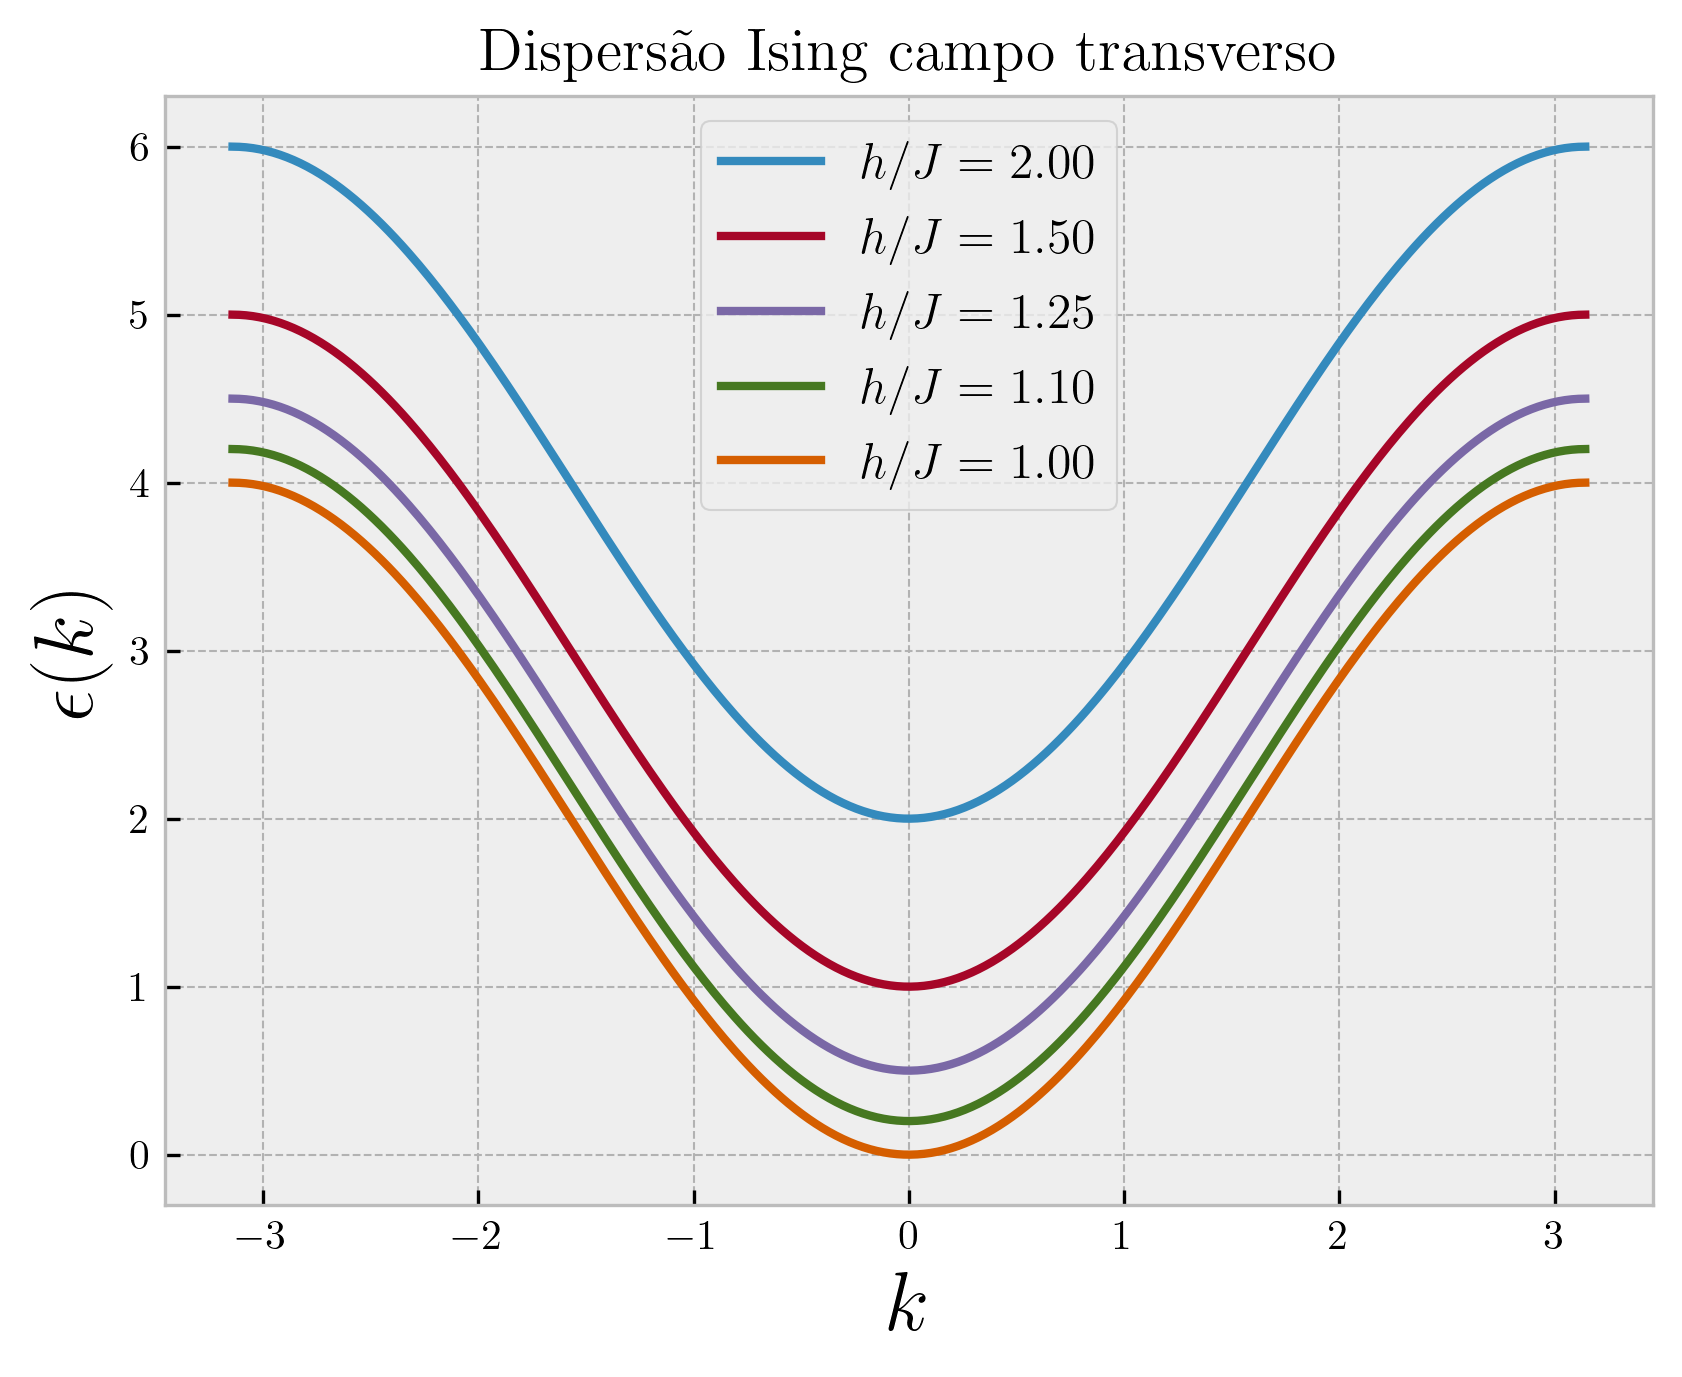
\includegraphics[width=0.8\linewidth]{fig/transv_ising.png}
\caption{Dispersão $\eps(k) = 2h - 2J \cos ka$ para várias razões $h/J$. Para $h/J = 1$, vemos que a curva fecha o gap (toca em zero). Os parâmetros utilizados no gráfico foram $J = a = 1$.}
\label{fig:transv_ising}
\end{figure}

\n

Podemos identificar o ponto crítico quântico como o ponto $h/J$ em que a dispersão $\eps(k)$ não possui gap com relação ao estado fundamental (em analogia com a transição condutor-isolante em Estado Sólido). Olhando a Figura \ref{fig:transv_ising}, vemos que isso acontece quando $h/J = 1$, onde o gap é fechado em $k = 0$. Assim, o ponto crítico quântico é $h = J$, o que está de acordo com a esquematização da Figura \ref{fig:qcp}.

\n\n

(c) Linearizando a hamiltoniana $H$ e desprezando as flutuações de segunda ordem para obter o campo médio ($\delta \s_j^x \, \delta \s_{j+1}^x \approx 0$), temos $\s_j^x = \ev{\s_j^x} + \delta \s_j^x = m_x + \delta \s_j^x$ e
$$
\s_j^x \s_{j+1}^x \approx -m_x^2 + m_x (\s_j^x + \s_{x+1}^x).
$$

\n

Substituindo na hamiltoniana $H$, obtemos a aproximação de campo médio
$$
H = J N m_x^2 - 2Jm_x \sum_{j} \s_j^x - h \sum_{j} \s_j^z = J N m_x^2 - \hhh \vdot \ss,
$$
onde $\hhh = (2J m_x, 0, h)$ e $\ss = \sum_{j} \ss_j = \sum_{j} \qty(\s_j^x, \s_j^y, \s_j^z)$.

\n

A função de partição de campo médio fica
$$
Z = \tr(e^{-\beta H}) = \sum_{\text{many-body states } \ket{\Psi}} \ev**{\exp(-\beta J N m_x^2 + \beta \hhh \vdot \ss)}{\Psi}
$$
$$
Z =
e^{-\beta J N m_x^2} \sum_{\text{many-body states } \ket{\Psi}} \ev**{\exp(\beta \hhh \vdot \ss)}{\Psi}.
$$

A soma acima é sobre todos os many-body states da forma
$$
\ket{\Psi} = \prod_{j=1}^N \ket{\psi_j},
$$
com os estados de partícula única $\ket{\psi_j} = \ket{\up}$ ou $\ket{\down}$. Dessa forma
$$
Z =
e^{-\beta J N m_x^2} \sum_{\text{many-body states } \ket{\Psi}} \ev**{\exp(\sum_{j} \beta \hhh \vdot \ss_j)}{\Psi} =
$$
$$
= e^{-\beta J N m_x^2} \sum_{\ket{\psi_j} = \ket{\up},\ket{\down}} \prod_j \ev**{\exp(\beta \hhh \vdot \ss_j)}{\psi_j} =
$$
$$
= e^{-\beta J N m_x^2} \prod_j \sum_{\ket{\psi_j} = \ket{\up},\ket{\down}} \ev**{\exp(\beta \hhh \vdot \ss_j)}{\psi_j} =
$$
$$
= e^{-\beta J N m_x^2} \qty{\sum_{\ket{\psi} = \ket{\up},\ket{\down}} \ev**{\exp[\beta \hhh \vdot (\s^x, \s^y, \s^z)]}{\psi}}^N
$$

Para calcular  $\ev**{\exp[\beta \hhh \vdot (\s^x, \s^y, \s^z)]}{\psi}$, lembre que a exponencial de um operador é
$$
e^A = \sum_{n=0}^{\infty} \frac{A^n}{n!} \implies
\ev**{e^A}{\psi} = \sum_{n=0}^{\infty} \frac{\ev**{A^n}{\psi}}{n!}.
$$

\n

Temos que
$$
\ev**{\beta \hhh \vdot \vecs}{\psi} =
\beta \ev**{(\hh_x \s_j^x + \hh_z \s_j^z)}{\psi} =
$$
$$
=
\beta \hh_x \cancelto{0}{\ev**{\s^x}{\psi}} +
\beta \hh_z \ev**{\s^z}{\psi} =
\begin{cases}
\; +\beta \hh_z, \quad \ket{\psi} = \ket{\up}, \\
\; -\beta \hh_z, \quad \ket{\psi} = \ket{\down}.
\end{cases}
$$
$$
[\beta \hhh \vdot \vecs]^2 = \beta^2 (\hh_x \s^x + \hh_z \s^z)^2 =
\beta^2 \Big[\hh_x^2 \cancelto{1}{(\s^{x})^2} + \hh_z^2 \cancelto{1}{(\s^{z})^2}
+ \hh_x \hh_z \cancelto{0}{\{\s^x, \s^z\}}\Big] =
\beta^2 (\hh_x^2 + \hh_y^2) = \qty(\beta \abs{\hhh})^2.
$$

Portanto, vale que
$$
\ev**{\Big[\beta \hhh \vdot \vecs\Big]^{2n}}{\psi} = \qty(\beta \abs{\hhh})^{2n},
$$
$$
\ev**{\Big[\beta \hhh \vdot \vecs\Big]^{2n+1}}{\psi} =
\begin{cases}
\; +\beta \hh_z \, \qty(\beta \abs{\hhh})^{2n}, \; \ket{\psi} = \ket{\up}, \\
\; -\beta \hh_z \, \qty(\beta \abs{\hhh})^{2n}, \; \ket{\psi} = \ket{\down}.
\end{cases}
$$

Esses resultados levam que
$$
\ev**{\exp[\beta \hhh \vdot (\s^x, \s^y, \s^z)]}{\up} +
\ev**{\exp[\beta \hhh \vdot (\s^x, \s^y, \s^z)]}{\down} =
2 \sum_{n=0}^{\infty} \frac{\qty(\beta \abs{\hhh})^{2n}}{(2n)!} = 2 \cosh(\beta\abs{\hhh}).
$$

Finalmente, obtemos
$$
\boxed{ Z = e^{-\beta J N m_x^2} \qty[2\cosh(\beta \abs{\hhh})]^N } \implies
\boxed{ f = -\frac{1}{\beta N} \log Z =
J m_x^2 - \frac{1}{\beta} \log\qty[2\cosh(\beta\sqrt{4J^2 m_x^2 + h^2})]. }
$$

\n

A magnetização $m_x = \ev{\s^x}$ é dada pelo mínimo da energia livre
$$
0 = \pdv{f}{m} =
2 J m_x - 4 J^2m_x \, \frac{\tanh(\beta\sqrt{4J^2 m_x^2 + h^2})}{\sqrt{4J^2 m_x^2 + h^2}} \implies
$$
$$
\sqrt{m_x^2 + \qty(\frac{h}{2J})^2} = \tanh(2 \beta J \sqrt{m_x^2 + \qty(\frac{h}{2J})^2}).
$$

Explorando esse resultado para $T = 0$, temos que $\beta \to +\infty$ e a tangente hiperbólica tende a $1$. Assim, para $T = 0$ temos
$$
\sqrt{m_x^2 + \qty(\frac{h}{2J})^2} = 1 \implies \boxed{ m_x = \sqrt{1 - \qty(\frac{h}{2J})^2}. }
$$

Note que para $m_x \to 0^+$ temos o ponto crítico quântico $h_c = 2J$, que é diferente do ponto crítico quântico $h = J$ que obtivemos no item (b).

\n

Expandindo $\sqrt{1+x} \approx 1 + \frac{1}{2}x$ para $m \to 0^+$ nos dá
$$
\frac{h}{2J} \, \sqrt{1 + \qty(\frac{2 m_x J}{h})^2} \approx
\frac{h}{2J} \qty(1 + \frac{2 m_x^2 J^2}{h^2}) = 1
\implies
$$
$$
\frac{h}{2J}  + \frac{m_x^2 J}{h} = 1 \implies
m_x = \sqrt{\qty(\frac{h}{J})\qty(1-\frac{h}{2J})}
$$
$$
m_x \approx \sqrt{2\qty(1-\frac{h}{2J})} \implies \boxed{ m_x \propto \qty(1-\frac{h}{2J})^{1/2}. }
$$

Assim, descobrimos o expoente crítico $\beta = 1/2$.

\n

A aproximação de campo médio nos dá o ponto crítico quântico $h_c = 2J$ e o expoente crítico $\beta = 1/2$. A referência \cite{pfeuty} faz o cálculo exato para este modelo em 1D e obtém  ponto crítico $h_c = J$ e o expoente $\beta = 1/8$. Assim, nosso resultado do item (b) $h_c = J$ está correto, enquanto percebemos que a aproximação de campo médio não é válida neste modelo em 1D. Isso é um fenômeno do próprio campo médio, pois só esperamos que ele nos dê o expoente crítico verdadeiro para dimensões maiores que a dimensão crítica superior do modelo, que neste caso é maior do que $d=1$.


%Definindo $y = \sqrt{m_x^2 + \qty(\frac{h}{2J})^2}$, temos que $y = \tanh(2\beta J y)$. Como vimos em aula, essa equação só tem solução $y \neq 0$ quando $2 \beta J > 1$, o que define a temperatura crítica $2 \beta_c J = 1 \implies T_c = 2J / k_B$.
%
%\n
%
%Para obter o expoente crítico $\beta$, expandimos a tangente hiperbólica em torno de zero para $T \to T_c$
%$$
%y = \tanh(\frac{T_c}{T} y) \approx \frac{T_c}{T} \, y - \frac{1}{3} \, \frac{T_c^3}{T^3} \, y^3 \implies
%y \approx \sqrt{3 \frac{(T_c-T)}{T_c}} \propto (T_c - T)^{1/2},
%$$
%o que nos dá o expoente crítico $\beta = 1/2$.
%
%\n
%
%A magnetização em função de $h$ perto do ponto crítico $T \to T_c$ fica
%$$
%m_x = \sqrt{3 \, \frac{T_c - T}{T_c} - \qty(\frac{h}{2J})^2}.
%$$
%
%\n
%
%Interpretando esta solução, percebemos que o campo $h$ (que é aplicado na direção $z$) tem o efeito contra a magnetização $m_x$, o que faz sentido físico pois se $h$ for grande os spins se alinharão na direção $z$, deixando a magnetização $m_x$ em zero. A magnetização $m_x$ só consegue ser maior que zero abaixo da temperatura crítica $T < T_c$ e se a fração $h/J$ for pequena. No caso do zero absoluto $T = 0$, o ponto crítico quântico é $h = J$, mas para $0 < T < T_c$ esse valor é diferente. Por exemplo, para $T$ perto de $T_c$, o ponto crítico quântico é
%$$
%3 \, \frac{T_c - T}{T_c} - \qty(\frac{h}{2J})^2 \to 0^+ \implies
%h = 2J \sqrt{\frac{3(T_c - T)}{T_c} } \propto J,
%$$
%que também é proporcional a $J$.


%%-----
%% Referências bibliográficas
%%-----
\addcontentsline{toc}{chapter}{\bibname}
%\bibliographystyle{abntex2-num}
\bibliography{citations}
\bibliographystyle{ieeetr}


\end{document}
